\documentclass[answers]{exam} %[answers]
\usepackage{xeCJK}
\usepackage{amsmath}
\usepackage{amssymb}
\usepackage{polynom}
\usepackage{ulem}
\usepackage{tikz}
\usepackage{tkz-euclide}
\title{七年级上数学错题整理}

\newcommand\epart{\part}

\newcommand\degree{^\circ}
\renewcommand{\solutiontitle}{\noindent\textbf{解:}\par\noindent}
\everymath{\displaystyle}
\usetkzobj{all}

\begin{document}
\maketitle

\section{重要考试}

\subsection{七年级阶段性诊断1}

\begin{questions}
\question
下列说法中,正确的有\fillin
  
\begin{oneparchoices}
  \choice $\frac{3 \pi xy}{5}$的系数是$\frac{3}{5}$;
  \correctchoice $-2^2ab^2$的次数是$5$;
  \choice 多项式$mn^2+2mn-3n-1$的次数是$3$;
  \choice $\pi - b$和$\frac{xy}{2}$都是整式。
\end{oneparchoices}

\question
阅读理解题

定义:
如果一个数的平方等于$-1$,记为$i^2=-1$,这个数叫做虚数单位。
那么和我们所学的实数对应起来就叫做复数,表示为$a+bi$(a,b为实数),$a$叫这个复数的实部,$b$叫做这个复数的虚部,
它的加,减,乘法运算与整式的加,减,乘法运算类似。

例如计算: $(2+i) + (3-4i)=5-3i$

\begin{parts}
\epart
填空: $i^3=$\fillin[$-i$],$i^4=$\fillin[$1$]

\epart
计算 
\begin{subparts}
\subpart $(2+i)(2-i)$
\vspace*{1in}
\begin{solution}
\[    
\begin{aligned}
  \mbox{原式} &= 4 - i^2 \\
  &= 5
\end{aligned}
\]  
\end{solution}

\subpart $(2 + i)^2$
\vspace*{1in}
\begin{solution}
\[    
\begin{aligned}
  \mbox{原式} &= 4 + 4i + i^2 \\
  &= 3 + 4i
\end{aligned}
\]  
\end{solution}

\end{subparts}

\epart
若两个复数相等,则它们的实部和虚部必须分别相等,完成下列问题

已知:$(x+y)+3i=(1-x)-yi$,($x$,$y$为实数),求$y$的值

\vspace*{1in}
\begin{solution}
\[
\begin{aligned}
& \because \mbox{若两个复数相等,则它们的实部和虚部必须分别相等} \\
& \therefore \begin{cases} x+y=1-x \\ 3i = -yi \end{cases} \\
& \therefore \begin{cases} y=-3 \\ x=2 \end{cases} \\
& \mbox{答} \begin{cases} x=2 \\ y=-3 \end{cases}
\end{aligned}
\]
\end{solution}

\epart
试一试:请利用以前学习的有关知识将$\frac{1+i}{1-i}$化简成$a+bi$的形式
  
\vspace*{1in}
\begin{solution}
\[
\begin{aligned}
  & \mbox{设} i - 1 \mbox{为} a \\
  & \begin{aligned}
    \mbox{原式} &= \frac{(1+i)^2}{(1 - i^2)} \\
    &= \frac{1 - 1 + 2i}{2} \\
    &= i
    \end{aligned}
\end{aligned}
\]
\end{solution}

\end{parts}

\end{questions}

\subsection{七年级期中} 

\begin{questions}
\question
如果关于x的不等式组$ \begin{cases} m-4x>4 \\ x-\frac{11}{2}<3(x+\frac{1}{2}) \end{cases} $有且仅有三个奇数解,
且关于x的方程式$ \frac{2-mx}{2-x}-\frac{30}{x-12}=13$有非负数解,
则符合条件的所有整数m的和是\fillin

\begin{oneparchoices}
  \choice 15
  \choice 27
  \correctchoice 29
  \choice 42
\end{oneparchoices}

\question
若$ 2^m=a,32^n=b $ , m、n为正整数,则$ 2^{3m-10n}$=\fillin[$ \frac{a^3}{b^2}$]

\question
A是关于x的二次整式,且二次项系数为1,A与多项式$(x+2)$相乘后的结果为两项的多项式,则A=\fillin[$x^2-2x$或$x^2$或$x^2-2x+4$]

\question
若关于x的方程$\frac{2x+m}{x-1}=3$的解为正整数,则m的取值范围是\fillin[$m>-3$且$m \neq -2$]

\question
我们知道,同底数幂的乘法为:$a^ma^n=a^{m+n}(其中a \neq 0, m,n为正整数)$,
类似地我们规定关于任意正整数m,n的一种新运算:$h(m+n)=h(m)h(n)$,请根据这种新运算填空:
\begin{parts}
  \epart 若$h(1)=\frac{2}{3}$,则$h{2}$=\fillin;
  \epart 若$h(1)=k(k \neq 0)$,那么$h(n) \cdot h(2017)$=\fillin(用含n和k的代数式表示,其中n为正整数)。
\end{parts}

\question
已知$a$、$b$、$c$、$n$是互不相等的正整数,且$\frac{1}{a}+\frac{1}{b}+\frac{1}{c}+\frac{1}{n}$也是整数,则$n$的最大值是\fillin[42]

\question
若一个自然数t能写成$t=x^2-y^2$($x$,$y$均为正整数,且$x \neq y$),则称$t$为“万象数”,
$x$、$y$为$t$的一个万象分解,在t的所有万象分解中,若$\frac{x-y}{x+y}$最小,则称$x$,$y$为$t$的一个万象分解,
在$t$的所有万象分解中,若$\frac{x-y}{x+y}$最小,则称$x$,$y$为$t$的绝对万象分解,此时$F(t)=\frac{x}{y}$。
例如:$32=9^2-7^2=6^2-2^2$,因为$\frac{9-7}{9+7}=\frac{1}{8}$,$\frac{6-2}{6+2}=\frac{1}{2}$,$\frac{1}{8}<\frac{1}{2}$,
所以$9$和$7$为$32$的绝对万象分解,此时$F(32)=\frac{9}{7}$。
若一个四位正整数,它的千位数字与个位数字相同,百位数字与十位数字相同,但四个数字不全相同,则称这个四位数位“博雅数”。例如$2001$,$4554$均为“博雅数”。
若一个四位正整数$m$是“万象数”且能被$13$整除,“博雅书” $n$ 的前两位数字组成的两位数与后两位数字组成的两位数恰好是$m$的一个万象分解,
则所有满足条件的数$m$中$F(m)$的最大值为\fillin[$\frac{64}{48}$]。

\question
把一张长方形纸先左右对折,再上下对折(记为对折 $2$ 次),然后再折叠着的角上剪刀,将纸展开后,纸的中间就剪出了一个洞。
把一张纸按“先左右、再上下”的顺序对折$6$次后,再在折叠着的角上剪一刀,将这张纸展开,请动手操作,纸上会出现\fillin[16]个洞。

\question
因式分解:$16(6x-1)(2x-1)(3x+1)(x-1)+25$

\vspace*{1in}
\begin{solution}
  \[
    \begin{aligned}
      \mbox{原式}
      & = 16(12x^2-8x+1)(3x^2-2X-1)+25{} \\
      & = 16(4t+1)(t-1)+25 \\
      & = 16(4t^2-3t=1)+25 \\
      & = 64t^2-48t+9 \\
      & = (8t-3)^2 \\
      & = (24x^2 - 16x -3)^2
    \end{aligned}
  \]
\end{solution}

\question
初中数学学习阶段,我们常常会利用一些变形技巧来化简式子,解答问题。

材料一:在解决分式问题时,倒数法是常用的变形技巧之一,所谓倒数法,即把式子变成其倒数形式,从而运用约分化简,以达到计算的目的

例,已知:$\frac{x}{(x^2+1)}=\frac{1}{4}$求代数式$x^2+\frac{1}{x^2}$的值。

解:
\[ Q \frac{x}{x^2+1}=\frac{1}{4},
  \therefore \frac{x^2+1}{x}=4 \mbox{即} \frac{x^2}{x}+\frac{1}{x}=4,
  \therefore x+\frac{1}{x}=4,
  \therefore x^2+\frac{1}{x^2}=(x+\frac{1}{x})^2-2=14
\]

材料二:在解决某些连等是问题问题时,通常可以引入参数“k”,将连等式变成几个值为k的等式,
这样就可以通过适当变形解决问题的值

例:若$2x=3y=4z$,且$xyz \neq 0$,求$\frac{x}{y+x}$的值。

解:
\[
  \mbox{令} 2x=3y=4z=k(k≠0),
  \mbox{则} x=\frac{k}{2},y=\frac{k}{3},z=\frac{k}{4},
  \therefore \frac{x}{y+z}=\frac{\frac{1}{2}k}{\frac{1}{3}k + \frac{1}{4}k}=\frac{\frac{1}{2}}{\frac{7}{12}}=\frac{7}{6}
\]

根据材料回答问题:

\begin{parts}

  \epart
  已知$\frac{x}{x^2-x+1}=\frac{1}{2}$,则$x+\frac{1}{x}=$\fillin[3]

  \epart
  若$\frac{yz}{bz+cy}=\frac{zx}{cx+az}=\frac{xy}{ay+bx}=\frac{x^2+y^2+z^2}{a^2+b^2+c^2}$,$x \neq 0$,$y \neq 0$,$z \neq 0$,且$abc=5$,
  求$xyz$的值

  \vspace*{1in}
  
  \begin{solution}
    \[
    \begin{split}
      \frac{y}{bz+cy}=\frac{x}{cx+az} \\
      \therefore \frac{bz+cy}{y}=\frac{cx+az}{x} \\
      \therefore \frac{bz}{y}=\frac{az}{y}
    \end{split}
  \]
  \end{solution}

\end{parts}

\end{questions}

\subsection{七年级阶段性诊断2}

\begin{questions}

\question
计算: $(x+y)(-x-y)$=\fillin[$-x^2-2xy-y^2$]

\question
解方程: $\frac{2x+2}{x+3}-\frac{5}{7}=\frac{x}{x+3}$

\vspace*{1in}
\begin{solution}
\[
\begin{aligned}
  14x+14-5x-15 &= 7x \\
  9x - 1 &= 7x \\
  x &= \frac{1}{2} \\
\end{aligned}
\]
经验算$x = \frac{1}{2}$为原方程的解
\end{solution}

\question
2019年下半年受各种因素的影响,猪肉市场价格不断上升。
据调查10月份猪肉的价格是9月份猪肉价格的1.25倍。
小英妈妈用50元钱在10月份购得的猪肉比在9月份购得的猪肉少0.4斤,求2019年9月份的每斤猪肉价格

\vspace*{1in}
\begin{solution}
  \[
\begin{aligned}
  & \mbox{设9月每斤猪肉$x$元,则10月为$1.25x$元。} \\
  & \begin{aligned}
  \frac{50}{1.25x}+0.4 &= \frac{50}{x} \\
  40 + 0.4x &= 50 \\
  0.4x &= 10 \\
  x &= 25 \\
  \therefore \mbox{原方程的解为} x = 25
  \end{aligned} \\
  & \mbox{答: 9月份每斤猪肉为25元} \\
  & \mbox{经验算,}x=25\mbox{为原方程的解,且符合题意}
\end{aligned}
\]
\end{solution}

\question 
如图,在直角三角形$ABC$中,$\angle B=90^{\degree}$,点$M$、$N$分别在边$BA$、$BC$上,且$BM=BN$。
  
\begin{parts}
\epart 画出直角三角形ABC关于直线MN堆成的三角形$A'B'C'$;
\epart 如果$AB=a,BC=b,BM=x$ 用$a$、$b$、$x$的代数式分别表示三角形$AMA'$的面积$S_1$和四边形$AA'C'C$的面积$S$,并简化。
\end{parts}

\begin{center}
\begin{tikzpicture}
  \tkzDefPoint[label=$A$](0,4){A}
  \tkzDefPoint[label=left:$B$](0,0){B}
  \tkzDefPoint[label=right:$C$](2,0){C}
  \tkzDefPoint[label=left:$N$](0,1){N}
  \tkzDefPoint[label=below:$M$](1,0){M}
  \tkzDrawPolygon(A,B,C)
  \tkzDrawPoints[](A,B,C,M,N)
\end{tikzpicture}
\end{center}

\vspace*{1in}
\begin{solution}
  
\begin{parts}
\epart
如$\triangle A'B'C'$就是所需要的三角形

\epart
\[
\begin{aligned}
  &
  \begin{aligned}
  S_{\triangle AMA}' &= \frac{ah}{2} \\
  &= \frac{(a-x)^2}{2} \\
  &= \frac{a^2-2ax+x^2}{2}
  \end{aligned} \\
  &
  \begin{aligned}
    S_{\Box AA'C'C} &= S_{\triangle AA'M} + S_{\triangle CNC'}+2S_{\triangle ABC}-S_{\Box MBNB'} \\
    &= \frac{(a-x)^2}{2} + \frac{(b-x)^2}{2} + ab - x^2 \\
    &= \frac{a^2 + 2x^2 + b^2 - 2x^2 +2ab - 2ax - 2bx}{2} \\
    &= a^2 + b^2 +2ab - 2ax - 2bx
  \end{aligned}
\end{aligned}
\]

\end{parts}

\end{solution}

\end{questions}

\subsection{数学达人赛}

\begin{questions}
\question
  已知$a^2-4a-1=0$,则$a^4+\frac{1}{a^4}=$\fillin[322]
  \vspace*{1in}
  \begin{solution}
    \[
      \begin{aligned}
        a^2 - 1 &= 4a \\
        a - \frac{1}{a} &= 4 \\
        (a + \frac{1}{a})^2 &= 16 \\
        a^2 + \frac{1}{a^2} - 2 &= 16 \\
        a^2 + \frac{1}{a^2} &= 18 \\
        a^4 + \frac{1}{a^4} + 2 &= 324 \\
        a^4 + \frac{1}{a^4} &= 322
      \end{aligned}
    \]
  \end{solution}

\question
  设$f(x) = (2x - 1)^5$,且展开式$f(x)=a_0 + a_1x + a_2x^2 + a_3x^3 +
  a_4x^4 + a_5x^5$,试求$\frac{2}{3}(a_1 + a_3)=$\fillin[$\frac{244}{3}$]
  \vspace*{1in}
  \begin{solution}
    \[
      \begin{aligned}
        & \begin{cases}
          \mbox{当} x = 1 \mbox{时} \quad a_0 + a_1 + a_2 + a_3 + a_4 = 1 \quad\textcircled{1} \\
          \mbox{当} x = 0 \mbox{时} \quad a_0 = -1 \quad\textcircled{2} \\
          \mbox{当} x = -1 \mbox{时} \quad a_0 - a_1 + a_2 - a_3 + a_4 = 243 \quad\textcircled{3}
        \end{cases} \\
        & \mbox{由} \textcircled{1} + \textcircled{3} \mbox{得} 244 = 2a_0 + a_2 + a_4 \\
        & a_2 + a_4 = 246 \\
        & \therefore a_1 + a_3 = 122
      \end{aligned}
    \]
  \end{solution}

\question
  已知$2^{(x-1)}+2^{(x-2)}+2^{(x-3)}=448$,则$x=$\fillin[9]

  \vspace*{1in}
  \begin{solution}
    \[
      \begin{aligned}
        x^{x-1}(1 + 2 + 4) &= 448 \\
        x^{x-1} &= 64 \\
        x &= 9
      \end{aligned}
    \]
  \end{solution}

\question
  从左到右的变形,时因式分解的为
  \begin{choices}
    \choice $ma+mb-c=m(a+b)-c$
    \choice $(a-b)(a^2+ab+b^2)=a^3-b^3$
    \choice $a^2-4ab+4b^2-1=a(a-4b)+(2b+1)(2b-1)$
    \choice $4x^2-25y^2=(2x+5y)(2x-5y)$
  \end{choices}

\question
  计算: $(-\frac{1}{2}x + 3)^2(-\frac{1}{2}x-3)^2-2(x-5)(x-2)$

  \vspace*{1in}
  \begin{solution}
    \[
      \begin{aligned}
        \mbox{原式} &= (\frac{1}{4}x^2 - 9)^2 - 2x^2 + 14x - 20 \\
        &= (\frac{1}{16}x^4 - \frac{9}{2}x^2 + 81) - 2x^2 + 14x - 20 \\
        &= \frac{1}{16}x^4 - \frac{13}{2}x^2 + 14x + 61
      \end{aligned}
    \]
  \end{solution}

\question
  已知$2^{10}=a^2=4^b$,先化简再求职:$(\frac{1}{4}a +
  \frac{1}{5}b)(\frac{1}{4}a-\frac{1}{5}b)-(\frac{1}{4}a+\frac{1}{5}b)^2$

  \vspace*{1in}
  \begin{solution}
    错在哪里?
    \[
      \begin{aligned}
        & \begin{aligned}
          \mbox{原式} &= (\frac{1}{4}a + \frac{1}{5}b)(-\frac{2}{5}b) \\
          &= - \frac{2b}{25} - \frac{ab}{10}
        \end{aligned} \\
        & \begin{aligned}
          \because  2^{10} &= a ^2 \\
          (2^5)^2 &= a^2 \\
          a &= 2^5
        \end{aligned}
        & \begin{aligned}
          2^{10} &= 4^b \\
          4^5 &= 4^{b} \\
          b &= 5
        \end{aligned} \\
        & \begin{aligned}
          \mbox{原式} &= - \frac{2*5^2}{25} - \frac{2^5*5}{10} \\
          &= -2 - 2^4 \\
          &= -18
        \end{aligned}
      \end{aligned}
    \]
  \end{solution}

\question
  已知:$x^4 + 6x^2 + x + 12$有一个因式是$x^2 + ax + 4$,求$a$值和这个
  多项式的其他因式。

  \vspace*{1in}
  \begin{solution}
    \[
      \begin{aligned}
        & \mbox{设另一个多项式是}x^2 + bx + 3 \mbox{,则} \\
        & \begin{aligned}
          \mbox{原式} &= (x^2 + ax + 4)(x^2 + bx + 3) \\
          &= x^4 + (a + b)x^3 + (3 + 4 + ab)x^2 + (3a + 4b)x + 12
        \end{aligned} \\
        & \therefore \begin{cases}
          a + b = 0 \qquad \textcircled{1} \\
          3 + 4 + ab = 6 \qquad \textcircled{2} \\
          3a + 4b = 1 \qquad \textcircled{3}
        \end{cases} \\
        & \mbox{由} \textcircled{1} \quad \textcircled{3} \mbox{得} \begin{cases}
          a = -1 \\ b = 1
        \end{cases} \\
        & \mbox{代入} \textcircled{2} \mbox{, 等式成立} \\
        & \therefore a  = -1 \mbox{, 另一个因式为} x^2 + x + 3
      \end{aligned}
    \]
  \end{solution}
\end{questions}

\section{周测}

\subsection{周测一}

\begin{questions}

\question
  如果$a^{n^2}=(a^n)^x$($n$为正整数),那么$x$等于
  
  \begin{choices}
  \correctchoice $n$
  \choice $2$
  \choice $a^n$
  \choice $a^2$
  \end{choices}

\question
  若$2x+5y-3=0$,则$4^x \cdot 32^y$的值为\fillin[8]

\question
  因式分解 $x^4-2(a^2+b^2)x^2+(a^2-b^2)^2$

  \vspace*{1in}
  \begin{solution}
    \[
      \begin{aligned}
        \mbox{原式} &= x^4-2(a^2+b^2)x^2+[(a+b)(a-b)]^2 \\
        &= (x^2)^2 - 2(a^2+b^2)x^2+(a+b)^2(a-b)^2 \\
        &= (x^2)^2-(2a^2+2b^2)x^2+(a^2+2ab+b^2)(a^2-2ab+b^2) \\
        &= [x^2-(a^2+2ab+b^2)] \cdot [x^2-(a^2-2ab+b^2)] \\
        &= [x^2-(a+b)^2] \cdot [x^2-(a-b)^2] \\
        &= (x+a+b)(x-a-b)(x+a-b)(x-a+b)
      \end{aligned}
    \]
  \end{solution}

\question
  因式分解 $(x^2+3x-2)(x^2+3x+4)-16$

  \vspace*{1in}
  \begin{solution}
\[
  \begin{aligned}
    \mbox{令} x^2+3x-2\mbox{为}a \\
    \mbox{原式} &= a(a+6)-16 \\
    &= (a-2)(a+8) \\
    &= (x^2+3x-4)(x^2+3x+6) \\
    &= (x - 1)(x + 4)(x^2 + 3x + 6)
  \end{aligned}
\]
\end{solution}

\question
  因式分解 $(xy+1)(x+1)(y+1)+xy$

  \vspace*{1in}
  \begin{solution}
\[
\begin{aligned}
  \mbox{原式} &= (xy+1)(xy+1+x+y)+xy \\
  &= t(t+x+y)+xy \\
  &= t^2+t(x+y)+xy \\
  &= (t+x)(t+y) \\
  &= (xy + 1 + x)(xy + 1 + y)
\end{aligned}
\]
\end{solution}

\question
  已知$(2000-a)(1998-a)=1999$,求$(2000-a^2)+(1998-a)^2$的值.

  \vspace*{1in}
  \begin{solution}
\[
\begin{aligned}
  \mbox{设} 2000 - a = m \quad 1998-a = n \\
  \begin{cases} m \cdot n =1999 \\ m - n = 2 \end{cases} \\
\end{aligned}
\]
\end{solution}

\question
  已知正有理数$a$、$b$、$c$满足方程
  $
    \begin{cases}
      a + b^2 + 2ac = 29 \quad\textcircled{1}\\
      b + c^2 + 2ab = 17 \quad\textcircled{2}\\
      c + a^2 + 2bc = 26 \quad\textcircled{3}\\
    \end{cases} 
  $
  求$a+b+c$的值

  \vspace*{1in}
  \begin{solution}
  \[
    \begin{aligned}
      & \mbox{由} \textcircled{1} + \textcircled{2} + \textcircled{3} \mbox{得} \\
      & \begin{aligned}
        a + b + c + a^2 + b^2 + c^2 + 2ab + 2ac + 2bc & = 72 \\
        a + b + c + (a + b + c)^2 &= 72 \\
        (a + b + c)(a + b + c + 1) &= 72 \\
      \end{aligned} \\
      & \because 72 = 8 * 9 \\
      & \therefore a + b + c = 8
    \end{aligned}
  \]
\end{solution}

\question
  对于多项式$x^3-5x^2+x+10$, 我们吧$x=2$代入多项式,发现$x=2$能使多项
  式$x^3-5x^2+x+10$的值为0,由此可以断定多项式$x^3-5x^2+x+10$中有因式
  $(x-2)$[注:把$x=a$代入多项式,能使多项式的值为0,则多项式一定含有因
  式$(x-a)$],于是我们可以把多项式写成$x^3-5x^2+x+10=(x-2)(x^2+mx+n)$,
  分别求出$m$,$n$后再代入$x^3-5x^2+x+10=(x-2)(x^2+mx+n)$,就可以把多
  项式$x^3-5x^2+x+10$因式分解。
  \begin{parts}
    \epart 求式子中$m$,$n$的值。
    \epart 以上这种因式分解的方法叫“试根法”,用“试跟法”分解多项式
    $x^3+5^2+8x+4$。
  \end{parts}

  \vspace*{1in}
  \begin{solution}
\begin{parts}
  \epart
  \[
    \begin{aligned}
      & x^3 - 5x^2 + x + 10 = (x - 2)(x^2 - 3x - 5) \\
      & \therefore \begin{cases} m = -3 \\ n = -5 \end{cases}
    \end{aligned}
    \polylongdiv{x^3 - 5x^2 + x + 10}{x - 2}
  \]

  \epart
  \[
    \begin{aligned}
      & \mbox{当} x = -1 \mbox{时值为0} \\
      & \therefore \mbox{一定含因式} x + 1 \\
      & \begin{aligned}
        x^3 + 5x^2 + 8x + 4 &= (x + 1)(x^2 + mx + n) \\
        &= (x + 1)(x^2 + 4x + 4)
      \end{aligned} \\
      & \therefore \begin{cases}
        m = 4 \\
        n = 4
      \end{cases} \\
      & \begin{aligned}
        \therefore \mbox{原式} &= (x + 1)(x^2 + 4x + 4) \\
        & = (x + 1)(x+2)^2
      \end{aligned}
    \end{aligned}
    \polylongdiv{x^3 + 5x^2 + 8x + 4}{x + 1}
  \]
\end{parts}
\end{solution}
  
\end{questions}

\subsection{周测二}

\begin{questions}
\question
  因式分解:$(m^2 + 3m)^2 - 8(m^2 + 3m) - 20=$\fillin[$(m-2)(m+2)(m-1)(m+5)$]

\question
  下列因式分解中正确的有
  \begin{itemize}
  \item $-2x^3-3xy^3+xy=-xy(2x^2-3y^2+1)$
  \item $-x^2 - y^2 = -(x+y)(x-y)$
  \item $16x^2 + 4y^2 - 16xy = 4(2x - y)^2$
  \item $x^2y + 2xy + 4y = y(x + 2)^2$
  \item $\frac{1}{2}x - y + x^2 - 4y^2 = \frac{1}{2}(x - 2y)(1 + 2x + 4y)$
  \end{itemize}

  \begin{oneparchoices}
    \choice 0 \choice 1 \correctchoice 2 \choice 3
  \end{oneparchoices}

\question
  计算: $\frac{2x^2}{x - 1} - x - 1$

  \vspace*{1in}
  \begin{solution}
    \[
      \begin{aligned}
        \mbox{原式} &= \frac{2x^2 - x^2 + 1}{x - 1} \\
        &= \frac{x^2 + 1}{x - 1}
      \end{aligned}
    \]
  \end{solution}

\question
  计算:
  $\frac{3}{(x + 1)(x + 3)} + \frac{3}{(x + 3)(x + 5)}
  + \frac{3}{(x + 5)(x + 7)} + \dots + \frac{3}{(x + 99)(x + 101)}
  $

  \vspace*{1in}
  \begin{solution}
    \[
      \begin{aligned}
        \mbox{原式} &= 3 * \frac{1}{2} ( \frac{1}{x + 1} - \frac{1}{x + 3} + \frac{1}{x + 3} \dots - \frac{1}{x + 101}) \\
        &= 3 * \frac{1}{2} * \frac{100}{(x + 1)(x + 101)} \\
        &= \frac{150}{(x + 1)(x + 101)}
      \end{aligned}
    \]
  \end{solution}

\question
  因式分解: $(x^2 - y^2)^2 - 8(x^2 + y^2) + 16$

  \vspace*{1in}
  \begin{solution}
    \[
      \begin{aligned}
        \mbox{原式} &= (x^2 - y^2)^2 - 8(x^2 - y^2) + 16 - 16 y^2 \\
        &= (x^2 - y^2 - 4)^2 - 16y^2 \\
        &= (x^2 - y^2 - 4 + 4y)(x^2 - y^2 - 4 - 4y) \\
        &= (x^2 - (y - 2)^2)(x^2 - (y + 2)^2) \\
        &= (x - y + 2)(x + y - 2)(x - y - 2)(x - y + 2)
      \end{aligned}
    \]
  \end{solution}

\question
  已知$\frac{1}{a^2} + \frac{1}{b^2} = \frac{4}{a^2 + b^2}$,求
  $(\frac{b}{a})^{2013} - (\frac{a}{b})^{2014}$的值?

  \vspace*{1in}
  \begin{solution}
    \[
      \begin{aligned}
        & \begin{aligned}
          \frac{1}{a^2} + \frac{1}{b^2} &= \frac{4}{a^2 + b^2} \\
          \frac{a^2 + b^2}{a^2 b^2} &= \frac{4}{a^2 + b^2} \\
          4 a^2 b^2 &= a^4 + b^4 + 2 a^2 b^2 \\
          (a^2 - b^2)^2 &= 0 \\
          a^2 &= b^2 \\
          a = b & \mbox{或} a = -b
        \end{aligned} \\
        & \therefore \begin{cases}
          \mbox{当} a = b \mbox{时} \qquad &\mbox{原式} = 0 \\
          \mbox{当} a = -b \mbox{时} \qquad &\mbox{原式} = -2
        \end{cases}
      \end{aligned}
    \]
  \end{solution}

\question
  定义: 如果一个分式能化成一个整式与一个分子为常数的分式的和的形式,则
  称这个分式为“和谐分式”。如
  $\frac{x+1}{x-1}
  =\frac{x - 1 + 2}{x - 1}
  =\frac{x - 1}{x - 1} + \frac{2}{x - 1}
  =1 + \frac{2}{x - 1}$,
  $\frac{2x- 3}{x + 1}
  = \frac{2x + 2 - 5}{x + 1}
  = \frac{2x + 2}{x + 1} + \frac{-5}{x + 1}
  = 2 + \frac{-5}{x + 1}$,
  则$\frac{x+1}{x-1}$和$\frac{2x-3}{x+1}$都是“和谐分式”。

  \begin{parts}
    \epart 下列分式中,属于“和谐分式的是” \fillin[\textcircled{1},
    \textcircled{2},\textcircled{4}](填序号);

    \textcircled{1}$\frac{x+1}{x}$;
    \textcircled{2}$\frac{2+x}{2}$;
    \textcircled{3}$\frac{x+2}{x+1}$;
    \textcircled{4}$\frac{y^2+1}{y^2}$.

    \epart 将“和谐分式”$\frac{a^2-2a+3}{a-1}$化成一个整式与一个分子为
    常数的分式的和的形式为:$\frac{a^2-2a+3}{a-1}=$\fillin[$a -
    1$]$+$\fillin[$\frac{2}{a-1}$];

    \epart 应用:先化简$
    \frac{3x+6}{x+1}-\frac{x-1}{x}
    \div \frac{x^2-1}{x^2+2x}$,并求$x$取什么整数时,该式的值为整数。
    
    \vspace*{1in}
    \begin{solution}
      \[
        \begin{aligned}
        & \begin{aligned}
          \mbox{原式} &= 3 + \frac{3}{x+1} - \frac{x-1}{x} * \frac{x(x+2)}{(x+1)(x-1)} \\
          &= 3 + \frac{3}{x+1} - \frac{x+2}{x+1} \\
          &= 3 + \frac{1-x}{x+1} \\
          &= 2 + \frac{2}{x+1}
        \end{aligned} \\
        & \therefore x + 1 = 2 \mbox{或} 1 \mbox{或} -1 \mbox{或} -2 \\
        & \therefore x = 1 \mbox{或} 0 \mbox{或} -2 \mbox{或} -3 \\
        & \mbox{代入原式验算} x = 0, x = -1, x = -2 \mbox{时无意义} \\
        & \therefore x \mbox{的取值为} -3
        \end{aligned}
      \]
    \end{solution}
    
  \end{parts}
  
\end{questions}

\subsection{周测三}

\begin{questions}

\question
  $4x^3 - 8x^2$,$2x^2 - 8$,$4x^2 - 4x - 8$中的公因式为
  \fillin[$2(x-2)$]

\question
  用黑白两种颜色的正方形纸片,按黑色纸片数量逐次加$1$的规律拼成一列图
  案:

  第$n$个图案还有白色纸片\fillin[$(3n+1)$]张.

\question
  若$x^2 + xy + y = 16$ 且 $y^2 + xy + x = 28$,则$x+y$的值为
  \fillin[$6 \mbox{或} -7$]

\question
  计算: $ \frac{(y-x)(z-x)}{(x - 2y + z)(x + y - 2z)}
  + \frac{(z-y)(x-y)}{(x + y -2z)}
  + \frac{(x-z)(y-z)}{(y + z - 2x)(x - 2y + z)}$

  \vspace*{1in}
  \begin{solution}
    \[
      \begin{aligned}
        & \mbox{令} x-y = a, y-z = b, z-x=c \\
        & \begin{aligned}
          \mbox{原式} &= \frac{-ca}{(a-b)(b-c)} + \frac{-ba}{(b-c)(c-a)} + \frac{-bc}{(c-a)(a-b)} \\
          &= - \frac{ ca(c-a) + ba(a-b) + bc(b-c) } {(a-b)(b-c)(c-a)} \\
          &= - \frac{ ac^2 - a^2c + a^2b - ab^2 + b^2c - bc^2 } {(a-b)(b-c)(c-a)} \\
        & \\
        \end{aligned} \\
        & \mbox{方法一: 简单方法,全部展开} \\
        & \begin{aligned}
          \mbox{原式} &= - \frac{ ac^2 - a^2c + a^2b - ab^2 + b^2c - bc^2 } {abc - b^2c - a^2b + ab^2 - ac^2 + bc^2 + a^2c - abc} \\
          &= - \frac{ ac^2 - a^2c + a^2b - ab^2 + b^2c - bc^2 } { - b^2c - a^2b + ab^2 - ac^2 + bc^2 + a^2c } \\
          &= 1
        \end{aligned} \\
        & \\
        & \mbox{方法二: 尝试凑出分母中的一项} \\
        & \begin{aligned}
          \mbox{原式} &= - \frac{ (b-c)a^2 + (c^2 - b^2)a + (b^2c - bc^2) }{(a-b)(b-c)(c-a)} \\
          &= - \frac{ (b-c)(a^2 - (b+c)a + bc) }{(a-b)(b-c)(c-a)} \\
          &= - \frac{ (b-c)(a^2 - ab - ac + bc) }{(a-b)(b-c)(c-a)} \\
          &= - \frac{ (b-c)(a(a - b) - c(a - b)) }{(a-b)(b-c)(c-a)} \\
          &= - \frac{ (b-c)(a - c)(a - b) }{(a-b)(b-c)(c-a)} \\
          &= 1
        \end{aligned} \\
      \end{aligned}
    \]
  \end{solution}

\question
  分解因式:$xy(x^2-y^2) + yz(y^2 - z^2) + zx(z^2 - x^2)$

  \vspace*{1in}
  \begin{solution}
    \[
      \begin{aligned}
        & \because (x^2 - y^2) + (y^2 - z^2) + (z^2 - x^2) = 0 \\
        & \therefore z^2 - x^2 = - (x^2 - y^2) - (y^2 - z^2) \\
        & \begin{aligned}
          \mbox{原式} &= xy(x^2 - y^2) + yz(y^2 - z^2) - zx(x^2 - y^2) - zx(y^2 - z^2) \\
          &= x(y - z)(x^2 - y^2) + z(y - x)(y^2 - z^2) \\
          &= x(y - z)(x + y)(x - y) + z(y - x)(y - z)(y + z) \\
          &= (y - z)(x - y)[x(x + y) - z(y + z)] \\
          &= (y - z)(x - y)(x^2 + xy - zy - z^2) \\
          &= (y - z)(x - y)[(x + z)(x - z) + y(x - z)] \\
          &= (y - z)(x - y)(x - z)(x + y + z)
        \end{aligned}
      \end{aligned}
    \]
  \end{solution}

\question
  如果$a+\frac{1}{b}=1$,$b+\frac{2}{c}=1$,求$c+\frac{2}{a}$的值

\end{questions}

\section{预习导航}

\subsection{16.1 二次根式预习导航}

\begin{questions}

\question
当$x$\fillin[$ \ge 1$]时,$\frac{\sqrt{x-1}}{\sqrt{x}}$有意义;
当$x$\fillin[$\ne 1 \mbox{且} x \ge 0$]时,$\frac{3\sqrt{x}}{1-\sqrt{x}}$有意义;
当$x$\fillin[$\ge 0 \mbox{且} x \ne 4$]时,$\frac{1}{\sqrt{x}-2}$有意义;
已知$\sqrt{a^2-2ab+b^2}=b-a$,则$a$\fillin[$\le$]$b$;
当x满足\fillin[$x \le \frac{1}{3} \mbox{且} x \ne 3$]时,$\frac{\sqrt{1-3x}}{| x | - 3} $ 有意义。

\question
简化二次根式 $a\sqrt{-\frac{a+1}{a^2}}$的结果是\fillin

  \begin{choices}
  \choice $\sqrt{-a-a}$
  \correctchoice $-\sqrt{-a-1}$
  \choice $\sqrt{a+1}$
  \choice $-\sqrt{-a+1}$
  \end{choices}
    
\question 化简 $x \sqrt{\frac{y}{x}} + y \sqrt{\frac{x}{y}}$

  \vspace*{1in}
  \begin{solution}
  \[
    \begin{aligned}
      \mbox{原式}
      & = x \sqrt{\frac{xy}{x^2}} + y \sqrt{\frac{xy}{y^2}} \\
      & = x \frac{\sqrt{xy}}{|x|} + y \frac{\sqrt{xy}}{|y|}
    \end{aligned}
      \begin{split}
      \because xy \ge 0 \\
      \therefore
      \begin{cases}
        x \ge 0, y \ge 0 \quad \mbox{原式} = 2 \sqrt{xy} \\
        x \le 0, y \le 0 \quad \mbox{原式} = - 2 \sqrt{xy}
      \end{cases}
    \end{split} 
\]
\end{solution}  

\end{questions}

\subsection{16.2(1) 最简二次根式预习导航}

\begin{questions}
  
\question 化简 $a\sqrt{\frac{1}{a^2}-\frac{1}{b^2}}$

\end{questions}

\subsection{16.2(2) 最简二次根式预习导航}

\begin{questions}

\question 下面说法正确的是
  \begin{choices}
  \choice 被开方数相同的二次根式是同类二次根式
  \choice $\sqrt{8}$与$\sqrt{80}$是同类二次根式
  \choice $\sqrt{2}$与$\sqrt{\frac{1}{50}}$不是同类二次根式
  \choice 同类二次根式是根指数为2的根式
  \end{choices}

\end{questions}

\subsection{16.3(2) 二次根式的运算预习导航(乘除)}

\begin{questions}
\question
计算:$3 \sqrt{5a} \cdot 2 \sqrt{10b}$=\fillin

\question
使等式$\sqrt{(x+1)(x-1)}=\sqrt{x-1} \cdot \sqrt{x+1}$成立的条件是\fillin

\end{questions}

\subsection{16.3(3) 二次根式的混合运算预习导航}

\begin{questions}

\question
已知$x=\frac{\sqrt{3}-\sqrt{2}}{\sqrt{3}+\sqrt{2}},y=\frac{\sqrt{3}+\sqrt{2}}{\sqrt{3}-\sqrt{2}}$,则$x^2+y^2$的值为\underline{\quad\quad}

\question
化简$(\sqrt{\frac{x}{y}-2\sqrt{\frac{y}{x}}}) \cdot \sqrt{xy} \cdot \frac{x+y}{x-2y}$=\underline{\quad\quad\quad\quad}

\question
解答$[\frac{4}{(\sqrt{a}+\sqrt{b})(\sqrt{a}-\sqrt{b})} + \frac{\sqrt{a}+\sqrt{b}}{\sqrt{ab}(\sqrt{b}-\sqrt{a})}] \div \frac{\sqrt{a}-\sqrt{b}}{\sqrt{ab}}$,其中$a=4,b=4$
  ~\\
  ~\\
  ~\\

\end{questions}   

\section{新竹}

\subsection{16.1(1) 二次根式}

\begin{questions}

\question 如果$\sqrt{1-2a}$有意义,那么a的取值范围是\underline{\quad\quad}

\question 化简: $\sqrt{x^2-6x+9} + \left| 1-x \right| (1<x<3)$
  ~\\
  ~\\

\end{questions}

\subsection{16.1(2) 二次根式}

\begin{questions}

  \question
  写出使下列等式成立的$x$的取值范围: $\sqrt{x^2(3-x)}=x \sqrt{3-x}$

  \question
  求下列各式成立时,$x$的取值范围: $\sqrt{\frac{2x-1}{3x+2}}=\frac{\sqrt{2x-1}}{\sqrt{3x+2}}$
  
  \question
  已知$\sqrt{a^3+3a^2}=-a\sqrt{a+3}$,求$a$的取值范围。

  \question
  $\sqrt{\frac{3-y}{3+y}}=\frac{\sqrt{3-y}}{\sqrt{3+y}}$成立的条件是\underline{\quad\quad}

\question 已知实数满足$|1-x|=1+|x|$,化简$\sqrt{x^2(x-1)^2}$.

\end{questions}

\section{十每}

\subsection{12月17}

\begin{questions}

\question
  $\frac{1}{3}\sqrt{75a} - 10 \sqrt{ab^4} - \frac{2}{a}\sqrt{3a^3} + ab^2 \sqrt{\frac{121}{a}} $

  \vspace*{1in}
  \begin{solution}
    \[
      \begin{aligned}
        \mbox{原式} &= \frac{5}{3} \sqrt{3a} - 10b^2 \sqrt{a} - \frac{2}{a} * a * \sqrt{3a} + 11b^2 \sqrt{a} \\
        &= b^2 \sqrt{a} - \frac{1}{3} \sqrt{3a}
      \end{aligned}
    \]
  \end{solution}

\question
  先化简,再求值: 已知
  $x = \frac{ 2 - \sqrt{3} }{ 2 + \sqrt{3} }$,
  $y = \frac{ 2 + \sqrt{3} }{ 2 - \sqrt{3} }$,
  求 $\frac{x + y}{x - y}$

  \vspace*{1in}
  \begin{solution}
    \[
      \begin{aligned}
        & \begin{aligned}
        x &= (2 - \sqrt{3})^2 \qquad y &= (2 + \sqrt{3})^2 \\
        &= 7 - 4 \sqrt{3} \qquad &= 7 + 4 \sqrt{3} \\
        \end{aligned} \\
        & \begin{aligned}
          \mbox{原式} &= \frac{7 - 4 \sqrt{3} + 7 + 4 \sqrt{3}}{7 - 4 \sqrt{3} - 7 - 4 \sqrt{3}} \\
          &= \frac{17}{- 8 \sqrt{3}} \\
          &= - \frac{7}{4 \sqrt{3}} \\
          &= - \frac{7 \sqrt{3}}{12}
        \end{aligned}
      \end{aligned}
  \]
  \end{solution}

\question
  如图,已知并排方式的正方形$ABCD$和正方形$BEFG$的变长分别为$m$、$n$
  $(m > n)$,$A$、$B$、$E$三点在一直线上,且正方形$ABCD$和正方形$BEFG$
  的面积之差为12。

\begin{center}
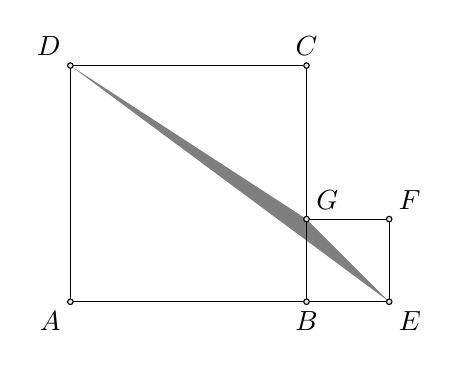
\begin{tikzpicture}[scale=1.5]
  \tkzDefPoint[label=below left:$A$](0,0){A}
  \tkzDefPoint[label=below:$B$](2,0){B}
  \tkzDefPoint[label=above:$C$](2,2){C}
  \tkzDefPoint[label=above left:$D$](0,2){D}
  \tkzDefPoint[label=below right:$E$](2.7,0){E}
  \tkzDefPoint[label=above right:$F$](2.7,0.7){F}
  \tkzDefPoint[label=above right:$G$](2,0.7){G}
  \tkzDrawPolygon(A,B,C,D)
  \tkzDrawPolygon(B,E,F,G)
  \tkzFillPolygon[opacity=0.5](D,G,E)
  \tkzDrawPoints[](A,B,C,D,E,F,G)
\end{tikzpicture}
\end{center}

\begin{parts}
  \epart 用含有$m$、$n$的代数式,表示涂红阴影部分的面积;
  \vspace*{1in}
  \begin{solution}
    \[
      \begin{aligned}
        S_{\mbox{阴影}} &= \frac{1}{2} S_{\Box BEFG} \\
        &= \frac{1}{2} n^2 \\
        &= \frac{n^2}{2}
      \end{aligned}
    \]
  \end{solution}

  \epart 连接$DB$、$CF$,则四边形$DGFC$的面积式多少?
  \vspace*{1in}
  \begin{solution}
    \[
      \begin{aligned}
        S_{\mbox{四边形}DGFC} &= \frac{(a+b)h}{2} \\
        &= \frac{(m+n)(m-n)}{2} \\
        &= \frac{m^2 - n^2}{2} \\
        &= \frac{12}{2} \\
        &= 6
      \end{aligned}
    \]
  \end{solution}
  
\end{parts}

\end{questions}

\subsubsection{12月18}

\begin{questions}
\question
  如图,已知$\triangle ABC$,将$\triangle ABC$沿直线$BC$平移得到
  $\triangle A_1B_1C_1$(其中 $A$、$B$、$C$ 分别与 $A_1$、$B_1$、$C_1$
  对应),平移的距离为$BC$长度的$\frac{2}{3}$。

\begin{center}
\begin{tikzpicture}[scale=1.0]
  \tkzDefPoints{-2.5/0/start, 5.5/0/end}
  \tkzDrawLines(start,end)

  \tkzDefPoints{1.2/1.7/A, 0/0/B, 3/0/C}
  \tkzDrawPolygon(A,B,C)
  \tkzLabelPoint[below](A){$A$}
  \tkzLabelPoint[below](B){$B$}
  \tkzLabelPoint[below](C){$C$}
  
  % \tkzDefShiftPoint[A](2,0){A1}
  % \tkzDefShiftPoint[B](2,0){B1}
  % \tkzDefShiftPoint[C](2,0){C1}
  % \tkzDrawPolygon(A1,B1,C1)
  % \tkzLabelPoint[below](A1){$A_1$}
  % \tkzLabelPoint[below](B1){$B_1$}
  % \tkzLabelPoint[below](C1){$C_1$}
  
\end{tikzpicture}
\end{center}

  \begin{parts}
    \epart 画出满足条件的$\triangle A_1B_1C_1$;
    \epart 联结$AC_1$,如果$\triangle ABC$的面积为$\frac{9}{2}$,求
    $\triangle ABC_1$的面积。
  \end{parts}

  \vspace*{1in}
  \begin{solution}
    \begin{enumerate}
    \item 向右移动
      \[
        \begin{aligned}
          & \because S_{\triangle ABC} : S_{\triangle ABC_{1}}  = 2 : 5 \\
          & \therefore S_{\triangle ABC_1} = \frac{15}{2}
        \end{aligned}
      \]
    \item 向左移动
      \[
        \begin{aligned}
          & \because S_{\triangle ABC} : S_{\triangle ABC_{1}}  = 3 : 1 \\
          & \therefore S_{\triangle ABC_1} = \frac{3}{2}
        \end{aligned}
      \]
    \end{enumerate}
  \end{solution}

\end{questions}

\subsubsection{21月19}

\begin{questions}
\question
  小明家到公园的路程为$38$千米,一天小明8点10分从家出发到公园游玩,他先步行
  了$1.5$千米然后换乘坐公交车,下车后又步行了$0.5$千米,9点40分到达公园.
  已知公交车的速度是小明步行速度的9倍,求小明步行的速度。

\question
  已知:如图所示,在$\triangle ABC$中

  \begin{parts}
    \epart 如果将$\triangle ABC$绕点$C$按顺时针方向旋转$90^{\degree}$
    得到$\triangle A_1B_1C$,点$A$、$B$分别与点$A_1$、$B_1$对应,
    请画出图形.(不要求写作图步骤)
    
    \epart 连接$A_1B$,$B_1B$,设$B_1B$与$A_1C$相交于点$O$。
    如果$AC⊥BB$,点$O$是线段$B_1B$的中点,
    且$\frac{S_{\triangle A_1B_1B}}{S_{\mbox{四边形}A_1B_1CB}} = \frac{1}{3}$,
    若$S_{\triangle A_1B_1B} = a$,试用含有$a$的代数式来表示$\triangle ABC$的面积。
  \end{parts}

\begin{center}
\begin{tikzpicture}[scale=2.0]
  \tkzDefPoints{0/0/C}
  \tkzDefShiftPoint[C](170:2.2){A}
  \tkzDefShiftPoint[C](125:2){B}
  \tkzDrawPolygon(A,B,C)
  \tkzLabelPoint[below](A){$A$}
  \tkzLabelPoint[below](B){$B$}
  \tkzLabelPoint[below](C){$C$}

  % \tkzDefShiftPoint[C](80:2.2){A1}
  % \tkzDefShiftPoint[C](35:2){B1}
  % \tkzDrawPolygon(A1,B1,C)
  % \tkzLabelPoint[below](A1){$A_1$}
  % \tkzLabelPoint[below](B1){$B_1$}
  
\end{tikzpicture}
\end{center}

\vspace*{1in}
\begin{solution}
  \begin{parts}
    \epart 如图就是所作的图
    \epart
    \[
      \begin{aligned}
        & \because \frac{S_{\triangle AB_1B}}{S_{\mbox{四边形}A_1B_1CB}} = \frac{1}{3} \\
        & \therefore S_{\mbox{四边形}A_1B_1CB} = 3a \\
        & \mbox{又} \because BO = B_1O \\
        & \therefore S_{\triangle A_1B_1C} = 1.5a = S_{\triangle ABC} \\
        & \therefore S_{\triangle ABC} \mbox{的面积为} 1.5a
      \end{aligned}
    \]
  \end{parts}
\end{solution}

\subsubsection{21月20}

\begin{questions}
\question
  甲乙两人玩“托球赛跑”游戏,商定:用球拍托着乒乓球从起跑线$L$起跑,到达
  $P$点后再返回起跑线为结束(如图所示);途中乒乓球掉下时须捡起并回到掉球
  处继续赛跑,所用时间少的人获胜。结果:甲同学由于心急,掉了球,浪费了6秒
  钟,乙同学则顺利跑完。事后,乙同学说:“我俩所用的全部时间的和为50秒”甲
  同学说:“不算掉球那段时间,我的速度是乙的1.2倍”,根据图文信息,请通过计
  算判定哪位同学获胜?

\begin{center}
\begin{tikzpicture}[scale=2.0]
  % \tkzDefPoints{0/0/C}
  % \tkzDefShiftPoint[C](170:2.2){A}
  % \tkzDefShiftPoint[C](125:2){B}
  % \tkzDrawPolygon(A,B,C)
  % \tkzLabelPoint[below](A){$A$}
  % \tkzLabelPoint[below](B){$B$}
  % \tkzLabelPoint[below](C){$C$}
\end{tikzpicture}
\end{center}

\vspace*{1in}
\begin{solution}
  \[
    \begin{aligned}
      & \mbox{设已为}\mbox{米/秒} \\
      & \begin{aligned}
        \frac{60}{1.2x} + 6 + \frac{60}{x} &= 50 \\
        50 + 6x + 60 &= 50x \\
        110 &= 44x \\
        x = \frac{5}{2}
      \end{aligned} \\
      & \mbox{经检验,} x = \frac{5}{2} \mbox{为方程组的解,且符合题意} \\
      & \therefore \mbox{原方程组的解为} x = \frac{5}{2} \\
      & \therefore \begin{cases}
        & 60 \div \frac{5}{2} = 24 (s) \\
        & 50 - 24 = 26 (s)
      \end{cases} \\
      & \therefore \mbox{乙胜} 
    \end{aligned}
  \]
\end{solution}

\end{questions}

\end{questions}

\end{document}

%%% Local Variables:
%%% End:
